% !TeX root = mercatormap.tex
% !TeX encoding=UTF-8
% !TeX spellcheck=en_US
% include file of mercatormap.tex (manual of the LaTeX package mercatormap)
\clearpage
\section{Automated Map Definition and Map Tiles}\label{sec:automated_map}%

\begin{center}
\begin{tikzpicture}[every node/.style={minimum width=3cm,minimum height=2cm,
  align=center,fill=red!5,draw=red!50!gray}]
\node (A) {Map Supply};
\node[at=(A.east),right=8mm] (B) {Python Script};
\node[at=(B.east),right=8mm] (C) {Map Apply};
\node[at=(C.east),right=8mm] (D) {Map Drawing};
\begin{scope}[->,very thick,Blue_Gray]
\draw (A)--(B); \draw (B)--(C); \draw (C)--(D);
\end{scope}
\end{tikzpicture}
\end{center}

As illustrated above, the script aided map definition is a process with
several stages.

\begin{itemize}
\item Map Supply: \refCom{mrcsupplymap} is the replacement of the manual setup by
  \refCom{mrcdefinemap}. Actually, it is quite similar to \refCom{mrcdefinemap}.
  With \refCom{mrcsupplymap} directions for the following Python script
  are formulated.
\item Python Script: The script is executed by \refCom{mrcsupplymap} during
  compilation. It does some coordinate system computations and downloads
  map tiles from a Web server. Finally, it writes a map definition into
  a file \meta{id}|.def|.
\item Map Apply: \refCom{mrcapplymap} reads and applies the
  map definition from \meta{id}|.def|.
\item Map Drawing: Afterwards, the map can be drawn by \refCom{mrcdrawmap}
  and other commands.
\end{itemize}

A map can be applied more than once, e.g. reused later in the document.
If this is not needed, map supply and map apply can be combined by
\refCom{mrcmap}.


%-------------------------------------------------------------------------------
\subsection{Script Activation}

Remember to install Python beforehand, see \Fullref{sec:python}.

\begin{docCommand}{mrcactivatescript}{}
  Use this inside the preamble of your document to activate the
  accompanying Python script.
  Without this command, the script is not executed!
  If the document is final (or the maps are final),
  this line could be removed and the document
  should be compilable without script.
\end{docCommand}


\begin{docMrcKey}{python}{=\meta{python}}{no default, initially |python|}
  Names the Python~3 interpreter as \meta{python}. If your Python~3 interpreter
  is not called |python|, but e.g. |python3|, then use
  \begin{dispListing}
  \mermapset{python=python3}
  \end{dispListing}
\end{docMrcKey}


\clearpage
%-------------------------------------------------------------------------------
\subsection{Map Types}
Currently, there are three methods provided how a map is computed by the
accompanying Python script. The technical background is documented in
\cite[Section~5]{Sturm:2020}.

\begin{enumerate}
\item \refKey{mermap/supply/type}|=|\docValue{reference}:
  \tcbsidebyside[sidebyside adapt=left,blankest,grow to left by=1cm]
  {
  \tikzexternaldisable
  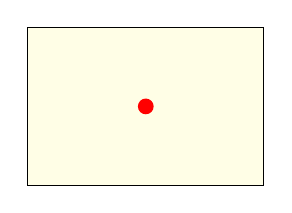
\begin{tikzpicture}
  \useasboundingbox (0,0) rectangle (3,2);
  \path[draw,fill=yellow!10] (0,0) rectangle (3,2);
  \path[fill=red] (1.5,1) circle [radius=1mm];
  \end{tikzpicture}
  }{
  The default method determines the map dimensions from a reference
  position and given document map dimensions.
  Also, a zoom level \refKey{mermap/supply/zoom}
  is required which relates to the Web Mercator map tile covering of the Earth.
  A higher zoom level gives a growing number of smaller map tiles.
  Alternative to the zoom level, a \meta{scale denominator} can be provided
  by \refKey{mermap/supply/flex area scale}, \refKey{mermap/flex scale}
  or \refKey{mermap/supply/flex reference scale} which determines
  the zoom level implicitly.
  As default, the reference position is the center of the map, but can be
  aligned at the map borders. This method is quite safe to use and could
  be the preferred one for many applications like showing the neighborhood
  of a route target.
  Finding the best reference point for depicting a certain area could
  be more tricky.
  }

\item \refKey{mermap/supply/type}|=|\docValue{areafit}:
  \tcbsidebyside[sidebyside adapt=left,blankest,grow to left by=1cm]
  {
  \tikzexternaldisable
  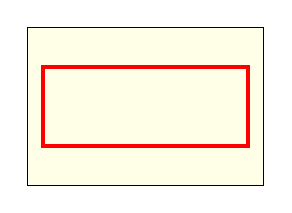
\begin{tikzpicture}
  \useasboundingbox (0,0) rectangle (3,2);
  \path[draw,fill=yellow!10] (0,0) rectangle (3,2);
  \path[draw=red,line width=0.5mm] (0.2,0.5) rectangle (2.8,1.5);
  \end{tikzpicture}
  }
  {
  The map dimensions are determined by an area with
  latitude and longitude boundaries which is fitted into given
  document map dimensions. The zoom level is computed accordingly
  for a fixed document tile size or by \refKey{mermap/supply/flex area fit}.
  In any case, the map contains the target area plus some protrusion.
  This method is also quite safe to use and may be
  the preferred one for many applications like showing a map which contains
  a bunch of markers (e.g. for locations of universities).
  If the map borders are required to exactly meet the boundaries,
  the third method can be regarded.
  }

\item \refKey{mermap/supply/type}|=|\docValue{boundaries}:
  \tcbsidebyside[sidebyside adapt=left,blankest,grow to left by=1cm]
  {
  \tikzexternaldisable
  
\begin{tikzpicture}
  \useasboundingbox (0,0) rectangle (3,2);
  \path[draw=red,line width=0.5mm,fill=yellow!10] (0.2,0.5) rectangle (2.8,1.5);
  \end{tikzpicture}
  }{
  The most obvious method determines the map dimensions from
  latitude and longitude boundaries. For this, a corresponding zoom level
  \refKey{mermap/supply/zoom}
  is required which relates to the Web Mercator map tile covering of the Earth.
  Alternative to the zoom level, a \meta{scale denominator} can be provided
  by \refKey{mermap/supply/flex area scale}
  or \refKey{mermap/supply/flex reference scale} which determines
  the zoom level implicitly.
  Note that a too high zoom level imposes the risk of downloading an unwanted
  high quantity of map tiles resulting in a much too large document map.
  Therefore, this most obvious method is \emph{not recommended} for the
  beginner and may be explored after some experience.
  }
\end{enumerate}



\clearpage
%-------------------------------------------------------------------------------
\subsection{Map Supply}

\begin{docCommand}{mrcsupplymap}{\oarg{options}\marg{definition}}
  The \meta{options} provide parameters for the Python~3 script to supply all
  materials for a map.
  All options share the common prefix |mermap/supply/|.\par
  The map is identified by\\
  \meta{id}=\refKey{mermap/definition prefix}+\meta{definition}\\
  for later drawing.
  This identifier \meta{id} has to be unique for the document.
  It corresponds to generated files \meta{id}|.def|, \meta{id}|.md5|, and
  possibly \meta{id}|.png|.
  Do not use spaces or special characters like umlauts for \meta{definition}.
  \par
  If \refCom{mrcactivatescript} is used inside the preamble,
  \refCom{mrcsupplymap} executes the Python~3 script, otherwise nothing happens.
\end{docCommand}


\begin{docCommand}{mermapsetsupply}{\marg{options}}
  Sets \meta{options} for all following maps inside the current \TeX\ group.
  All options share the common prefix |mermap/supply/|, e.g. for setting
  \refKey{mermap/supply/type} use
  \begin{dispListing}
    \mermapsetsupply{type=reference}
  \end{dispListing}
  Also see \refCom{mermapset} and \refCom{mermapsetmarker}.
\end{docCommand}


\begin{docMrcKey}{definition prefix}{=\meta{definition prefix}}{no default, initially |maps/|}
  Prefix for map identifiers and generated map files, see \refCom{mrcsupplymap}
  and \refCom{mrcapplymap}.
  Note that \refKey{mermap/definition prefix} is not to be used inside
  the option list for \refCom{mrcsupplymap}.
\end{docMrcKey}

\begin{docMrcKey}[supply]{type}{=\meta{type}}{no default, initially |reference|}
  The \meta{type} defines the basic computation for the map. Feasible values are
  \begin{itemize}
  \item\docValue{reference}: \flqq map with reference position\frqq\\
    The map is constructed from a given reference position
    \refKey{mermap/supply/latitude},\\
    \refKey{mermap/supply/longitude},\\
    a zoom level \refKey{mermap/supply/zoom},\\
    map dimensions\\
    \refKey{mermap/supply/width},\\
    \refKey{mermap/supply/height},\\
    and alignment \refKey{mermap/supply/align}.
  \item\docValue{areafit}: \flqq map fitting an area\frqq\\
    The map is constructed from a given area boundaries\\
    \refKey{mermap/supply/west},\\
    \refKey{mermap/supply/east},\\
    \refKey{mermap/supply/north},\\
    \refKey{mermap/supply/south},\\
    map dimensions\\
    \refKey{mermap/supply/width},\\
    \refKey{mermap/supply/height},\\
    and alignment \refKey{mermap/supply/align}.
  \item\docValue{boundaries}: \flqq map with boundaries\frqq\\
    The map is constructed from given boundaries\\
    \refKey{mermap/supply/west},\\
    \refKey{mermap/supply/east},\\
    \refKey{mermap/supply/north},\\
    \refKey{mermap/supply/south},\\
    and zoom level \refKey{mermap/supply/zoom}.
  \end{itemize}
\end{docMrcKey}

\pagebreak

\begin{docMrcKey}[supply]{zoom}{=\meta{setup zoom}}{no default, initially |9|}
  Map tile zoom factor alias $z$ coordinate of the map tiles.
  Used for map types \docValue{boundaries} and \docValue{reference}.
\end{docMrcKey}

\begin{docMrcKey}[supply]{north}{=\meta{setup north latitude}}{no default, initially |50|}
  Northern latitude degree, possibly negative for the southern hemisphere,
  lower than $90$ but always larger than \refKey{mermap/supply/south}.
  Used for map types \docValue{boundaries} and \docValue{areafit}.
\end{docMrcKey}

\begin{docMrcKey}[supply]{south}{=\meta{setup south latitude}}{no default, initially |48|}
  Southern latitude degree, possibly negative for the southern hemisphere,
  larger than $-90$ but always lower than \refKey{mermap/supply/north}.
  Used for map types \docValue{boundaries} and \docValue{areafit}.
\end{docMrcKey}

\begin{docMrcKey}[supply]{west}{=\meta{setup west longitude}}{no default, initially |11|}
  Western longitude degree, possibly negative for the western hemisphere,
  possibly shifted periodically, but always lower than \refKey{mermap/supply/east}.
  Used for map types \docValue{boundaries} and \docValue{areafit}.
\end{docMrcKey}

\begin{docMrcKey}[supply]{east}{=\meta{setup east longitude}}{no default, initially |13|}
  Eastern longitude degree, possibly negative for the western hemisphere,
  possibly shifted periodically, but always larger than \refKey{mermap/supply/west}.
  Used for map types \docValue{boundaries} and \docValue{areafit}.
\end{docMrcKey}


\begin{docMrcKeys}[
  doc keypath     = supply,
  doc parameter   = {=\marg{comma separated list of named positions}},
  doc description = {no default},
  %doc new         = 2020-05-04,
]{
  { doc name = area },
  { doc name = add area },
}
  Sets
  \refKey{mermap/supply/north}, \refKey{mermap/supply/south},
  \refKey{mermap/supply/west}, \refKey{mermap/supply/east}
  according to the given \meta{comma separated list of named positions}, i.e.
  the described area contains all these positions.\\
  \refKey{mermap/supply/area} resets the current area which requires
  at least two points inside the list.\\
  \refKey{mermap/supply/add area} does not reset the current area,
  i.e. the positions are added to the
  current area which possibly grows to fit all positions.\\
  Also note to take special care, if the international dateline is on your
  resulting map, see \Fullref{sec:dateline}.
  Used for map types \docValue{boundaries} and \docValue{areafit}
  or in combination with \refKey{mermap/supply/area to reference} also
  for for map type \docValue{reference}.
\end{docMrcKeys}



\begin{docMrcKeys}[
  doc keypath     = supply,
  doc parameter   = {=\marg{file name}},
  doc description = {no default},
  doc new         = 2020-05-08,
]{
  { doc name = area from marker input },
  { doc name = add area from marker input },
}
  Sets
  \refKey{mermap/supply/north}, \refKey{mermap/supply/south},
  \refKey{mermap/supply/west}, \refKey{mermap/supply/east}
  according to the given \refCom{mrcmarker} positions contained in a
  file with the given \meta{file name}.\\
  \refKey{mermap/supply/area from marker input} resets the current area which requires
  at least two marker positions inside the file.\\
  \refKey{mermap/supply/add area from marker input} does not reset the current area,
  i.e. the positions are added to the
  current area which possibly grows to fit all positions.\\
  Also note to take special care, if the international dateline is on your
  resulting map, see \Fullref{sec:dateline}.
  Used for map types \docValue{boundaries} and \docValue{areafit}
  or in combination with \refKey{mermap/supply/area to reference} also
  for for map type \docValue{reference}.
\end{docMrcKeys}



\begin{docMrcKey}[supply]{area to reference}{}{no value, initially unset}
  The map settings
  \refKey{mermap/supply/north}, \refKey{mermap/supply/south},
  \refKey{mermap/supply/west}, \refKey{mermap/supply/east}
  are taken to compute the map center. This center position is saved
  to \refKey{mermap/supply/latitude} and \refKey{mermap/supply/longitude}.
  Used for map type \docValue{reference}.
\end{docMrcKey}


\clearpage

\begin{docMrcKey}[supply]{latitude}{=\meta{setup latitude}}{no default, initially |49|}
  Latitude degree of a reference point, possibly negative for the southern hemisphere.
  Used for map type \docValue{reference}.
\end{docMrcKey}

\begin{docMrcKey}[supply]{longitude}{=\meta{setup longitude}}{no default, initially |12|}
  Longitude degree of a reference point, possibly negative for the western hemisphere.
  Used for map type \docValue{reference}.
\end{docMrcKey}


\begin{docMrcKey}[supply]{position}{=\meta{setup latitude}:\meta{setup longitude}}{no default, initially |49:12|}
  Latitude degree and longitude of a reference point.
  Used for map type \docValue{reference}.
\end{docMrcKey}


\begin{docMrcKey}[supply]{named position}{=\meta{name}}{style, no default}
  The \emph{named position} given by \meta{name} describes
  a reference point, see \Fullref{sec:names_positions}.
  Used for map type \docValue{reference}.
\end{docMrcKey}



\begin{docMrcKey}[supply]{width}{=\meta{setup width in tiles}}{no default, initially |4|}
  Width of the map as multiplicity of map tiles.
  Used for map types \docValue{reference} and \docValue{areafit}.
\end{docMrcKey}

\begin{docMrcKey}[supply]{tex width}{=\meta{width}}{style, no default}
  Width of the map as \TeX\ dimension.
  This is a style to compute \refKey{mermap/supply/width} according to
  the current \refKey{mermap/tile size}.
\end{docMrcKey}

\begin{docMrcKey}[supply]{height}{=\meta{setup height in tiles}}{no default, initially |4|}
  Height of the map as multiplicity of map tiles.
  Used for map types \docValue{reference} and \docValue{areafit}.
\end{docMrcKey}

\begin{docMrcKey}[supply]{tex height}{=\meta{width}}{style, no default}
  Height of the map as \TeX\ dimension.
  This is a style to compute \refKey{mermap/supply/height} according to
  the current \refKey{mermap/tile size}.
\end{docMrcKey}

\begin{docMrcKey}[supply]{align}{=\meta{setup alignment}}{no default, initially |center|}
  Alignment of reference point or area for map types \docValue{reference} and \docValue{areafit}.
  Feasible values are
  \docValue{northwest}, \docValue{north}, \docValue{northeast}, \docValue{west},
  \docValue{center}, \docValue{east}, \docValue{southwest},\docValue{south}, \docValue{southeast}.
\end{docMrcKey}

\begin{docMrcKey}[supply]{target}{=\meta{setup target}}{no default, initially |tiles|}
  Defines the type of output for the Python~3 script. Feasible values are:
  \begin{itemize}
  \item\docValue{none}: No tiles are downloaded and no merged map is generated, just map computation.
    This is the fastest method and needs no tile supplier.
  \item\docValue{tiles}: Download map tiles from a tile map service (TMS) \refKey{mermap/supply/url}.
    Compilation of a document with map tile takes longer than compilation
    with a merged map and transparency should not be used with tiles,
    but the resulting document is smaller than a document with merged maps.
  \item\docValue{mergedmap}: Download map tiles from a tile map service (TMS)
    \refKey{mermap/supply/url} and merge them into a single map picture.
    This speeds compilation and allows transparency effects, but
    the resulting document is possibly larger than a document with map tiles,
    because map tiles often are optimized 8-bit image files while the merged
    image is a 24-bit PNG file. Additionally, synergy effects of using the same map tiles
    for different maps are lost.
    Also, since the pixel map is clipped to full pixels, the resulting map
    may differ (shift/size) from the more accurate tile representation by
    one pixel.
  \item\docValue{wmsmap}: Download a single map from a web map service (WMS)
    \refKey{mermap/supply/url}. Internally, the package treats a WMS like
    a tile map service including all tile calculations. Actually, a single
    file is downloaded.
  \end{itemize}
\end{docMrcKey}

\enlargethispage*{1cm}

\begin{docMrcKey}[][doc new=2020-08-06]{fail on missing resource}{\colOpt{=true\textbar false}}{default |true|, initially |true|}
  If set to |true|, compilation stops with an error, if
  \refKey{mermap/supply/target} and \refKey{mermap/mapdef/resource} are different.
  Typically, this means that something went wrong while trying to download
  map tiles. Set this option temporarily to |false|,
  if the map tile service or the internet
  connection is expected to be unavailable only temporarily.
\end{docMrcKey}



\clearpage
\begin{docMrcKey}[supply]{url}{=\meta{setup URL}}{no default, initially empty}
  Here, the url format with placeholder |{z}{x}{y}| for map tile download is defined.
  \textbf{Be sure that you have the permission to download, save, and use
  the map tiles from that URL. Illegal downloads are not endorsed in any
  way.}
  \begin{dispListing}
    url={https://abc.efg.hij/{z}/{x}/{y}.png?apikey=12345678},
  \end{dispListing}
  See \Fullref{sec:maptileserver} for predefined URLs.
\end{docMrcKey}


\begin{docMrcKey}[supply]{url with api key}{=\marg{prefix}\marg{name}\marg{postfix}}{no default}
  This is an alternative version of \refKey{mermap/supply/url}.
  The URL is constructed from some fixed \meta{prefix} and \meta{postfix} with
  an API key in between. The API key is retrieved by \meta{name} from a
  repository filled by \refCom{mrcsetapikey}.
  \begin{dispListing}
    url={https://abc.efg.hij/{z}/{x}/{y}.png?apikey=}{myservice}{},
  \end{dispListing}
  See \Fullref{sec:maptileserver} for predefined URLs.
\end{docMrcKey}


\begin{docCommand}{mrcsetapikey}{\marg{name}\marg{value}}
  Stores an API key \meta{value} for access with the given \meta{name}.
  Typically, \meta{value} is a received ID from a map tile service provider
  after personal registration. \meta{name} is a placeholder which is used
  inside \refKey{mermap/supply/url with api key} to mark the insertion
  point for the API key.
  \begin{dispListing}
    \mrcsetapikey{myservice}{....K942XY....}
  \end{dispListing}
\end{docCommand}



\begin{docMrcKey}[supply]{attribution}{=\meta{attribution text}}{no default, initially empty}
  Attribution text for the map source. Typically, it acknowledges the copyright
  of the map data provider. It may contain hyperlinks.
  It is used to set up \refKey{mermap/mapdef/attribution} afterwards
  and it is accessible as \docAuxCommand{mrcmapattribution} (use read-only).\par
  For technical reasons, do not use \verb+"+. \docAuxCommand{mrcumlaut}
  may be used for masking umlauts, e.g. use \verb+\mrcumlaut{u}+ instead of
  \verb+\"{u}+, but umlauts can also be used directly, e.g. as UTF-8 coded characters.
\end{docMrcKey}

\begin{docMrcKey}[supply]{attribution print}{=\meta{attribution text}}{no default, initially empty}
  Attribution text for the map source.
  In contrast to \refKey{mermap/supply/attribution} it is intended for media
  that does not support hyperlinks like printed posters, books, etc.
  It is used to set up \refKey{mermap/mapdef/attribution print} afterwards
  and it is accessible as \docAuxCommand{mrcmapattributionprint} (use read-only).
\end{docMrcKey}


\begin{docMrcKey}[supply]{basename}{=\meta{setup tile base name}}{no default, initially \texttt{tiles/tile}}
  Prefix for local tile files, e.g. '|tiles/map|' for '|tiles/map_10_10_10.png|'.
\end{docMrcKey}


\clearpage
\begin{docMrcKey}[supply]{flex reference scale}{=\meta{scale denominator}}{no default}
  With the given \meta{scale denominator}, an appropriate \refKey{mermap/supply/zoom}
  and \refKey{mermap/tile size} is computed. Note that
  the \meta{scale denominator}
  always applies to the current \refKey{mermap/supply/latitude}
  and is used for map type \docValue{boundaries} and \docValue{reference}.
  For example, if the reference point is on the north side of the map,
  also the \meta{scale denominator}
  applies to the most northern latitude.

  Note to take special care to the order of the options.
  \begin{itemize}
  \item The reference point has to be set \emph{before}
    \refKey{mermap/supply/flex reference scale}, e.g. by
    \refKey{mermap/supply/latitude}, \refKey{mermap/supply/position},
    \refKey{mermap/supply/named position}.
  \item \refKey{mermap/supply/tex height}, \refKey{mermap/supply/tex width}
    (only for map type \docValue{reference})
    have to be set \emph{after} \refKey{mermap/supply/flex reference scale},
    because the \refKey{mermap/tile size} is adapted.
  \end{itemize}
  Also see \refKey{mermap/flex tile size}, \refKey{mermap/flex zoom},
  and \refKey{mermap/flex scale}.
\tikzsetnextfilename{maptiles_flex_reference_scale}%
\begin{dispExample}
\begin{tikzpicture}
  \mrcmap[type=reference,latitude=48.14,longitude=11.57,
    flex reference scale=250000,
    source=opentopomap,
    tex width=\linewidth,tex height=5cm]{}
  \mrcdrawmap
  \node[below,font=\fontsize{7pt}{7pt}\sffamily] at (mrcmap.south)
        {\mrcmapattribution};
  \mrcclipmap
  \path[draw] (mrcmap.south west) rectangle (mrcmap.north east);
  \node[below left=2mm,align=right,fill=white,fill opacity=0.5,
    text opacity=1] at (mrcmap.north east) {scale \mrcprettymapscale};
\end{tikzpicture}
\end{dispExample}
\end{docMrcKey}


\begin{docMrcKey}[supply]{flex area scale}{=\meta{scale denominator}}{no default}
  This is a shortcut for setting \refKey{mermap/supply/area to reference}
  and \refKey{mermap/supply/flex reference scale}=\meta{scale denominator}.
  Used for map type \docValue{boundaries} and \docValue{reference}.

  Note to take special care to the order of the options.
  \begin{itemize}
  \item The reference point has to be set \emph{before}
    \refKey{mermap/supply/flex area scale}.
  \item \refKey{mermap/supply/tex height}, \refKey{mermap/supply/tex width}
    (only for map type \docValue{reference})
    have to be set \emph{after} \refKey{mermap/supply/flex reference scale}.
  \end{itemize}
\end{docMrcKey}


\clearpage
\begin{docMrcKey}[supply]{flex area fit}{\colOpt{=\meta{size}}}{default |0pt|}
  This key can be used for map type \docValue{areafit} as \emph{final}
  option \emph{after} all other options.
  It applies a fine tuning to \refKey{mermap/tile size},
  \refKey{mermap/supply/width}, and \refKey{mermap/supply/height} such
  that the defined area fits exactly into the map region.
  If a \meta{size} is specified, width and height are reduced for the
  calculation by this \meta{size}, e.g. \meta{size}|=1cm| ensures a
  border of |5mm| on each side.
  Also see \refKey{mermap/flex tile size} and \refKey{mermap/flex zoom}.

\tikzsetnextfilename{maptiles_flex_area_fit}%
\begin{dispExample}
\begin{tikzpicture}
  \mrcNPdef{munich}{48.14}{11.58}
  \mrcNPdef{rio}{-22.91}{-43.20}
  \mrcNPdef{newyork}{40.71}{-74.01}
  \mrcmap[  type = areafit, area = {munich,rio,newyork},
    source=topplusopen web grau,
    tex width=\linewidth, tex height=7cm,
    flex area fit=1cm ]{}
  \mrcdrawmap
  \node[below,font=\fontsize{7pt}{7pt}\sffamily] at (mrcmap.south)
        {\mrcmapattribution};
  \draw[yellow] ([xshift=5mm,yshift=5mm]mrcmap.south west) rectangle
                ([xshift=-5mm,yshift=-5mm]mrcmap.north east);
  \draw[red,fill=red!50!gray!50!white,fill opacity=0.25]
    (\mrcNPcs{newyork}) -- (\mrcNPcs{rio}) -- (\mrcNPcs{munich}) -- cycle;
\end{tikzpicture}
\end{dispExample}
\end{docMrcKey}




\clearpage
\begin{docMrcKey}[supply]{pixel}{=\meta{setup pixel size}}{no default, initially |256|}
  Pixel width (and height) of a tile. It is especially needed for
  target \docValue{mergedmap} and also \docValue{wmsmap}.
  For \docValue{wmsmap}, it is multiplied with a pseudo tile calculation
  to compute the actual picture size to download.
\end{docMrcKey}


\begin{docMrcKey}[supply]{dpi}{=\meta{dpi value}}{style, no default}
  This style sets \refKey{mermap/supply/pixel} such that the given \meta{dpi value}
  is resulting (approximately).
  \begin{itemize}
  \item Note that this only applies for WMS Servers and not for
    TMS (Tile Map Service) Servers,
    because there \refKey{mermap/supply/pixel} is a fixed number depending on
    Server settings and cannot be chosen arbitrarily.
  \item A high \meta{dpi value} results in large downloaded map files.
    If the server does not provide a high resolution map, you will get
    unnecessary large files with blurred content.
  \item The \meta{dpi value} for TMS data can be changed by adapting
    \refKey{mermap/tile size} or \refKey{mermap/flex tile size}.
  \end{itemize}

\tikzsetnextfilename{maptiles_dpi_value}
\begin{dispExample}
\begin{tikzpicture}
 \mrcmap[type=reference,latitude=48.14,longitude=11.57,
    flex reference scale=250000,
    source=topplusopen p250, target=wmsmap, dpi=300,
    tex width=\linewidth,tex height=5cm]{dpi_value}
  \mrcdrawmap
  \node[below,font=\fontsize{7pt}{7pt}\sffamily] at (mrcmap.south)
        {\mrcmapattribution};
  \mrcclipmap
  \path[draw] (mrcmap.south west) rectangle (mrcmap.north east);
\end{tikzpicture}
\end{dispExample}

\end{docMrcKey}





%-------------------------------------------------------------------------------
\subsection{Map Apply}

\begin{docCommand}{mrcapplymap}{\marg{definition}}
  A map which is supplied by \refCom{mrcsupplymap} is applied
  inside a |tikzpicture| environment by
  \refCom{mrcapplymap} where \meta{definition} identifies the map.
  \refCom{mrcapplymap} replaces a manual setup by \refCom{mrcdefinemap}.
  The same map can be applied more than once inside a document.
  Note that applying a map does not mean to draw the map, but to prepare
  everything for drawing.
\end{docCommand}


\begin{docCommand}{mrcmap}{\oarg{options}\marg{definition}}
  This is a combination of
  \refCom{mrcsupplymap} with the given \meta{options}
  followed immediately by \refCom{mrcapplymap}.
  If \meta{definition} is left empty, an automated unique identifier is
  inserted.
  If a map is to be used just once, \refCom{mrcmap} may be preferred.
\end{docCommand}





\clearpage
%-------------------------------------------------------------------------------
\subsection{Map Tile Server}\label{sec:maptileserver}


To use map tiles with this package you obviously need access to a map tile server.
Thanks to all the many contributors to
\href{https://openstreetmap.org/copyright}{OpenStreetMap},
map data is free for everyone to use.
\textbf{But, map tile servers based on OpenStreetMap are not necessarily free}.

A list of online raster tile servers based on OpenStreetMap data is found here:\\
\url{https://wiki.openstreetmap.org/wiki/Raster_tile_providers}

\begin{itemize}
\item\bfseries I do not run a map tile server.
\item I do not and cannot grant any permission to access a map tile server.
\item I do not and cannot grant any permission to use map tiles in
  private, academic, free, or commercial publications.
\item All operators of map tile servers require to mention an attribution
  for their maps.
\end{itemize}

The following option allows easy usage of very few selected tile servers.
The tile server of \href{https://openstreetmap.org/copyright}{OpenStreetMap}
is not included because of its
\href{https://operations.osmfoundation.org/policies/tiles/}{Tile Usage Policy}.
I am aware that the following list could be enlarged much more, but I do not
want to add more to avoid any legal uncertainties.

\begin{itemize}
\item\bfseries I will remove an entry immediately, if the tile server operator
  asks for it.
\item\mdseries If \textbf{YOU} operate a tile server and you want an entry here, I would be
  glad to add it to the following list.
\end{itemize}

\medskip
\begin{docMrcKey}[supply]{source}{=\meta{source}}{style, no default}
  This style sets \refKey{mermap/supply/url}, \refKey{mermap/supply/attribution},\\
  \refKey{mermap/supply/attribution print} and \refKey{mermap/supply/basename}.\\
  Feasible values for \meta{source} are:
  %\mermapset{tile size=3.2512cm}
  \newcommand{\mapexample}[3][]{%
    \begingroup
    \mermapset{supply/source=#2}%
    \begin{itemize}
    \item Required attribution (\docAuxCommand{mrcmapattribution}):
      \begin{tcolorbox}[sharp corners,size=fbox,colback=yellow!8,colframe=yellow!80!gray,halign=flush left,before skip=2pt]
        \mrcmapattribution\end{tcolorbox}
    \item Required attribution for media without hyperlinks (\docAuxCommand{mrcmapattributionprint}):
      \begin{tcolorbox}[sharp corners,size=fbox,colback=yellow!8,colframe=yellow!80!gray,halign=flush left,before skip=2pt]
        \mrcmapattributionprint\end{tcolorbox}
    %\par\smallskip\
    \end{itemize}
    \endgroup\par\smallskip\tikzsetnextfilename{maptiles_#3}%
    \begin{tikzpicture}
    \mrcmap[source=#2,
      type=reference,latitude=48.14,longitude=11.58,zoom=7,
      tex width=\linewidth,tex height=2cm,#1]{#3}
      \mrcdrawmap
      \node[below,font=\fontsize{7pt}{7pt}\sffamily] at (mrcmap.south)
        {\mrcmapattribution};
    \end{tikzpicture}\par%
  }%
  \begin{itemize}

  \item\docValue{dummy}:\\
    Dummy tile server at loopback |127.0.0.1| for test purposes.

  \item\docValue{opentopomap}:\\
    Tile server (TMS) of \href{https://opentopomap.org/}{OpenTopoMap}.
    \begin{itemize}
    \item Usage (German language): \url{https://opentopomap.org/about#verwendung}
    \end{itemize}
    \mapexample{opentopomap}{opentopomap}

\clearpage
  \item\docValue{thunderforest opencyclemap}:\\
    Tile server of \href{https://www.thunderforest.com}{Thunderforest}.\\
    A registered \meta{api-key} is needed (free plan available)
    which is applied by\\
    \refCom{mrcsetapikey}\brackets{\docValue{thunderforest}}\marg{api-key}.
    \begin{itemize}
    \item Usage: \url{https://www.thunderforest.com/terms}
    \item API documentation: \url{https://www.thunderforest.com/maps/opencyclemap}
    \end{itemize}
    \mapexample{thunderforest opencyclemap}{thunderforest_opencyclemap}

  \item\docValue{thunderforest transport}:\\
    Tile server of \href{https://www.thunderforest.com}{Thunderforest}.\\
    A registered \meta{api-key} is needed (free plan available)
    which is applied by\\
    \refCom{mrcsetapikey}\brackets{\docValue{thunderforest}}\marg{api-key}.
    \begin{itemize}
    \item Usage: \url{https://www.thunderforest.com/terms}
    \item API documentation: \url{https://www.thunderforest.com/maps/transport}
    \end{itemize}
    \mapexample{thunderforest transport}{thunderforest_transport}

  \item\docValue{thunderforest landscape}:\\
    Tile server of \href{https://www.thunderforest.com}{Thunderforest}.\\
    A registered \meta{api-key} is needed (free plan available)
    which is applied by\\
    \refCom{mrcsetapikey}\brackets{\docValue{thunderforest}}\marg{api-key}.
    \begin{itemize}
    \item Usage: \url{https://www.thunderforest.com/terms}
    \item API documentation: \url{https://www.thunderforest.com/maps/landscape}
    \end{itemize}
    \mapexample{thunderforest landscape}{thunderforest_landscape}

\clearpage
  \item\docValue{thunderforest outdoors}:\\
    Tile server of \href{https://www.thunderforest.com}{Thunderforest}.\\
    A registered \meta{api-key} is needed (free plan available)
    which is applied by\\
    \refCom{mrcsetapikey}\brackets{\docValue{thunderforest}}\marg{api-key}.
    \begin{itemize}
    \item Usage: \url{https://www.thunderforest.com/terms}
    \item API documentation: \url{https://www.thunderforest.com/maps/outdoors}
    \end{itemize}
    \mapexample{thunderforest outdoors}{thunderforest_outdoors}

  \item\docValue{thunderforest atlas}:\tcbdocmarginnote{\tcbdocnew{2024-07-29}}\\
    Tile server of \href{https://www.thunderforest.com}{Thunderforest}.\\
    A registered \meta{api-key} is needed (free plan available)
    which is applied by\\
    \refCom{mrcsetapikey}\brackets{\docValue{thunderforest}}\marg{api-key}.
    \begin{itemize}
    \item Usage: \url{https://www.thunderforest.com/terms}
    \item API documentation: \url{https://www.thunderforest.com/maps/atlas}
    \end{itemize}
    \mapexample{thunderforest atlas}{thunderforest_atlas}

  \item\docValue{thunderforest transport-dark}:\\
    Tile server of \href{https://www.thunderforest.com}{Thunderforest}.\\
    A registered \meta{api-key} is needed (free plan available)
    which is applied by\\
    \refCom{mrcsetapikey}\brackets{\docValue{thunderforest}}\marg{api-key}.
    \begin{itemize}
    \item Usage: \url{https://www.thunderforest.com/terms}
    \item API documentation: \url{https://www.thunderforest.com/maps/transport-dark}
    \end{itemize}
    \mapexample{thunderforest transport-dark}{thunderforest_transport-dark}

\clearpage
  \item\docValue{thunderforest spinal-map}:\\
    Tile server of \href{https://www.thunderforest.com}{Thunderforest}.\\
    A registered \meta{api-key} is needed (free plan available)
    which is applied by\\
    \refCom{mrcsetapikey}\brackets{\docValue{thunderforest}}\marg{api-key}.
    \begin{itemize}
    \item Usage: \url{https://www.thunderforest.com/terms}
    \item API documentation: \url{https://www.thunderforest.com/maps/spinal-map}
    \end{itemize}
    \mapexample{thunderforest spinal-map}{thunderforest_spinal-map}

  \item\docValue{thunderforest pioneer}:\\
    Tile server of \href{https://www.thunderforest.com}{Thunderforest}.\\
    A registered \meta{api-key} is needed (free plan available)
    which is applied by\\
    \refCom{mrcsetapikey}\brackets{\docValue{thunderforest}}\marg{api-key}.
    \begin{itemize}
    \item Usage: \url{https://www.thunderforest.com/terms}
    \item API documentation: \url{https://www.thunderforest.com/maps/pioneer}
    \end{itemize}
    \mapexample{thunderforest pioneer}{thunderforest_pioneer}

  \item\docValue{thunderforest mobile-atlas}:\\
    Tile server of \href{https://www.thunderforest.com}{Thunderforest}.\\
    A registered \meta{api-key} is needed (free plan available)
    which is applied by\\
    \refCom{mrcsetapikey}\brackets{\docValue{thunderforest}}\marg{api-key}.
    \begin{itemize}
    \item Usage: \url{https://www.thunderforest.com/terms}
    \item API documentation: \url{https://www.thunderforest.com/maps/mobile-atlas}
    \end{itemize}
    \mapexample{thunderforest mobile-atlas}{thunderforest_mobile-atlas}

\clearpage
  \item\docValue{thunderforest neighbourhood}:\\
    Tile server of \href{https://www.thunderforest.com}{Thunderforest}.\\
    A registered \meta{api-key} is needed (free plan available)
    which is applied by\\
    \refCom{mrcsetapikey}\brackets{\docValue{thunderforest}}\marg{api-key}.
    \begin{itemize}
    \item Usage: \url{https://www.thunderforest.com/terms}
    \item API documentation: \url{https://www.thunderforest.com/maps/neighbourhood}
    \end{itemize}
    \mapexample{thunderforest neighbourhood}{thunderforest_neighbourhood}

  \item\docValue{topplusopen web}:\\
    Tile server (TMS) of \href{https://www.bkg.bund.de}{Bundesamt f\"{u}r Kartographie und Geod\"{a}sie}.
    \begin{itemize}
    \item Covers world / Europe / Germany depending on zoom level
    \item Usage (German language): \url{https://gdz.bkg.bund.de/index.php/default/digitale-geodaten/topplusopen-produkte.html}
    \end{itemize}
    \mapexample{topplusopen web}{topplusopen_web}

  \item\docValue{topplusopen web grau}:\\
    Tile server (TMS) of \href{https://www.bkg.bund.de}{Bundesamt f\"{u}r Kartographie und Geod\"{a}sie}.
    \begin{itemize}
    \item Covers world / Europe / Germany depending on zoom level
    \item Usage (German language): \url{https://gdz.bkg.bund.de/index.php/default/digitale-geodaten/topplusopen-produkte.html}
    \end{itemize}
    \mapexample{topplusopen web grau}{topplusopen_web_grau}

\clearpage
  \item\docValue{topplusopen web light}:\tcbdocmarginnote{\tcbdocnew{2024-07-29}}\\
    Tile server (TMS) of \href{https://www.bkg.bund.de}{Bundesamt f\"{u}r Kartographie und Geod\"{a}sie}.
    \begin{itemize}
    \item Covers world / Europe / Germany depending on zoom level
    \item Usage (German language): \url{https://gdz.bkg.bund.de/index.php/default/digitale-geodaten/topplusopen-produkte.html}
    \end{itemize}
    \mapexample{topplusopen web light}{topplusopen_web_light}

  \item\docValue{topplusopen web light grau}\tcbdocmarginnote{\tcbdocnew{2024-07-29}}:\\
    Tile server (TMS) of \href{https://www.bkg.bund.de}{Bundesamt f\"{u}r Kartographie und Geod\"{a}sie}.
    \begin{itemize}
    \item Covers world / Europe / Germany depending on zoom level
    \item Usage (German language): \url{https://gdz.bkg.bund.de/index.php/default/digitale-geodaten/topplusopen-produkte.html}
    \end{itemize}
    \mapexample{topplusopen web light grau}{topplusopen_web_light_grau}

\end{itemize}


\vfill
\begin{tcolorbox}[spartan,colback=white]
The following sources are Web map server (WMS). Therefore,
\refKey{mermap/supply/target} can only be set to \docValue{wmsmap}
or \docValue{none}.
\end{tcolorbox}
\clearpage

\begingroup
\ExplSyntaxOn
\int_gzero:N \g_tmpa_int
\NewDocumentCommand \cleanstep {}
{
  \fp_compare:nNnT { \g_tmpa_int-trunc(\g_tmpa_int/3)*3 } = 0
    {
      \int_compare:nNnT \g_tmpa_int > 0
        {
          \clearpage
        }
    }
  \int_gincr:N \g_tmpa_int
}
\ExplSyntaxOff

  \begin{itemize}

\foreach \name / \scdenom / \xtra in {p5/5000,p10/10000,p17.5/17500,p25/25000,p50/50000,p100/100000,p250/250000}
{
\cleanstep
  \item\docValue{topplusopen \name}:\\
    Web map server (WMS) of \href{https://www.bkg.bund.de}{Bundesamt f\"{u}r Kartographie und Geod\"{a}sie}.
    \begin{itemize}
    \item 1:\scdenom, covers Europe / Germany depending on zoom level
    \item Usage (German language): \url{https://gdz.bkg.bund.de/index.php/default/digitale-geodaten/topplusopen-produkte.html}
    \end{itemize}
    \mapexample[target=wmsmap]{topplusopen \name}{topplusopen_\name}

\cleanstep
  \item\docValue{topplusopen \name\ grau}:\\
    Web map server (WMS) of \href{https://www.bkg.bund.de}{Bundesamt f\"{u}r Kartographie und Geod\"{a}sie}.
    \begin{itemize}
    \item 1:\scdenom, covers Europe / Germany depending on zoom level
    \item Usage (German language): \url{https://gdz.bkg.bund.de/index.php/default/digitale-geodaten/topplusopen-produkte.html}
    \end{itemize}
    \def\grau{ grau}%
    \mapexample[target=wmsmap]{topplusopen \name\grau}{topplusopen_\name_grau}
}

  \end{itemize}
\endgroup

\end{docMrcKey}



\begin{docCommand}{mrcnewsupplysource}{\marg{source}\marg{options}}
  Adds a new \meta{source} value to \refKey{mermap/supply/source}.
  The \meta{options} should set the keys
  \refKey{mermap/supply/url}, \refKey{mermap/supply/attribution},\\
  \refKey{mermap/supply/attribution print} and \refKey{mermap/supply/basename}.
  It is recommend to use |x ...| for \meta{source} to avoid conflicts
  with future official additions to \refKey{mermap/supply/source}.
  \begin{dispListing}
  \mrcnewsupplysource{x example}
  {
    url               = https://127.0.0.1/dummy/{z}/{x}/{y}.png,
    attribution       = {Dummy tile server},
    attribution print = {Dummy tile server},
    basename          = tiles/dummy,
  }
  \end{dispListing}
\end{docCommand}


